\documentclass[../main.tex]{subfiles}
	% ELECTRONICS TESTING
\begin{document}

BLABLABLA.
\todo[inline,color=blue!20]{Write Electro Testing}

%%%%%%%%%%%%%%%%%%%%%%%%%%%%%%%%%%%%%%%%%%%%%%%%%%%%%%%%%%%%%%%%%%%%%%%%%%%%%%%%%%%%%%%%%%%%%%%%%%%%%%%%%%%%%%%%%%%%%%%%%%%%%%%%%%

\section{Electrical Characteristics of the Raspberry Pi}

Benchmarking

\begin{figure}[ht]
	\centering
	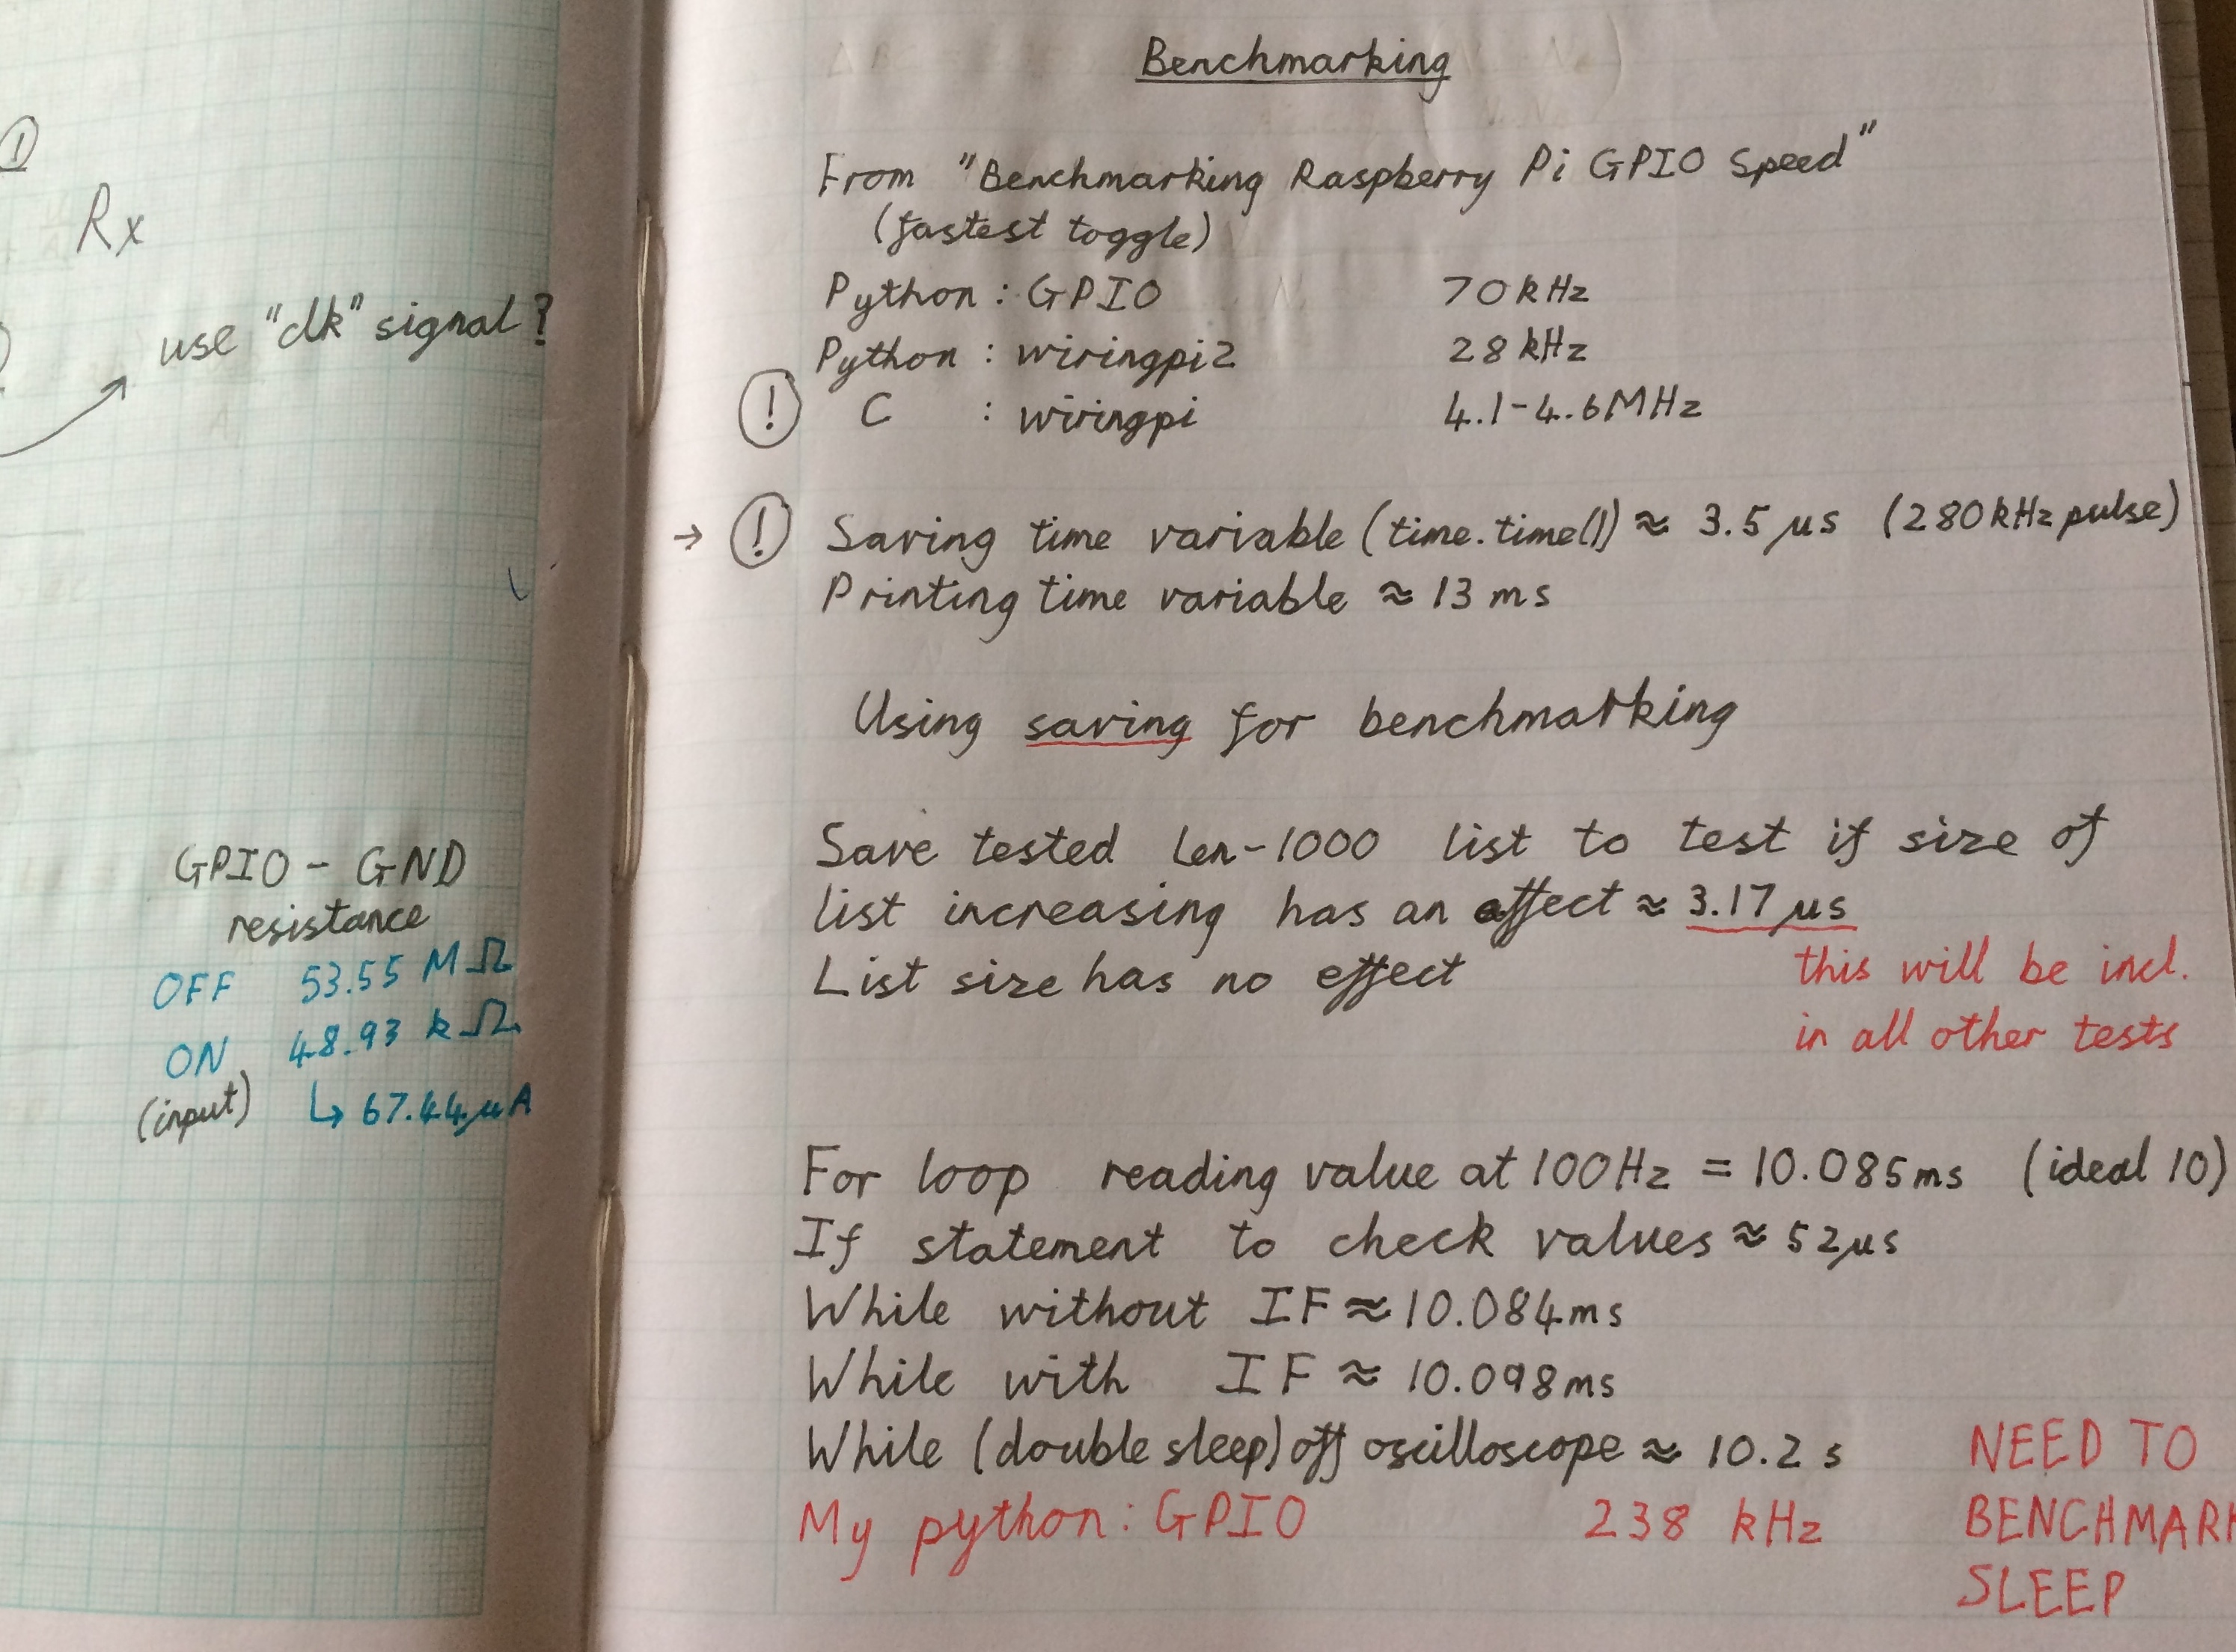
\includegraphics[width=0.6\textwidth]{Benchmarking_Data.jpg}
	\caption{Remove once written up}
	%\label{fig_}
\end{figure}

\todo[inline]{Include data collected in Interim report AND SCREENSHOTS IN IMAGES FILE}

\subsection{Impedance}

%%%%%%%%%%%%%%%%%%%%%%%%%%%%%%%%%%%%%%%%%%%%%%%%%%%%%%%%%%%%%%%%%%%%%%%%%%%%%%%%%%%%%%%%%%%%%%%%%%%%%%%%%%%%%%%%%%%%%%%%%%%%%%%%%%

\section{Compuational Characteristics of the Raspberry Pi} \label{sec_Computation}

time.time() in for loop - 3.32 us
time.time() in while loop with i++ - 4.02 us = slower
time.time() sequential - 2.81 us
therefore for loop time - 0.51us

100Hz (excluding the 10ms)
sleep(1/freq) - 104.13 us
sleep(1/freq-timeDif) - 90.08 us == REMOVES DELAY OF ~15us - GPIO AND A BIT
SAME without sleep(1/freq) (just GPIO) - 5.18 us
SAME without GPIO.output (just sleep(1/freq)) - 97.18 us == SLEEP IS THE INEFFICIENT FUNCTION LOSING ME TIME
You can hard-code in the ~104e-6 value to get offset of ~5us instead of 104us but this is not ideal - need to compare to coding in c...

\subsection{Maximum Frequency}

\todo[inline,color=blue!20]{Comparison of transmitter bank vs individual write and receiver read (callback) and read vars on clock pulse vs bank read on clock pulse}

\begin{figure}[ht]
	\centering
	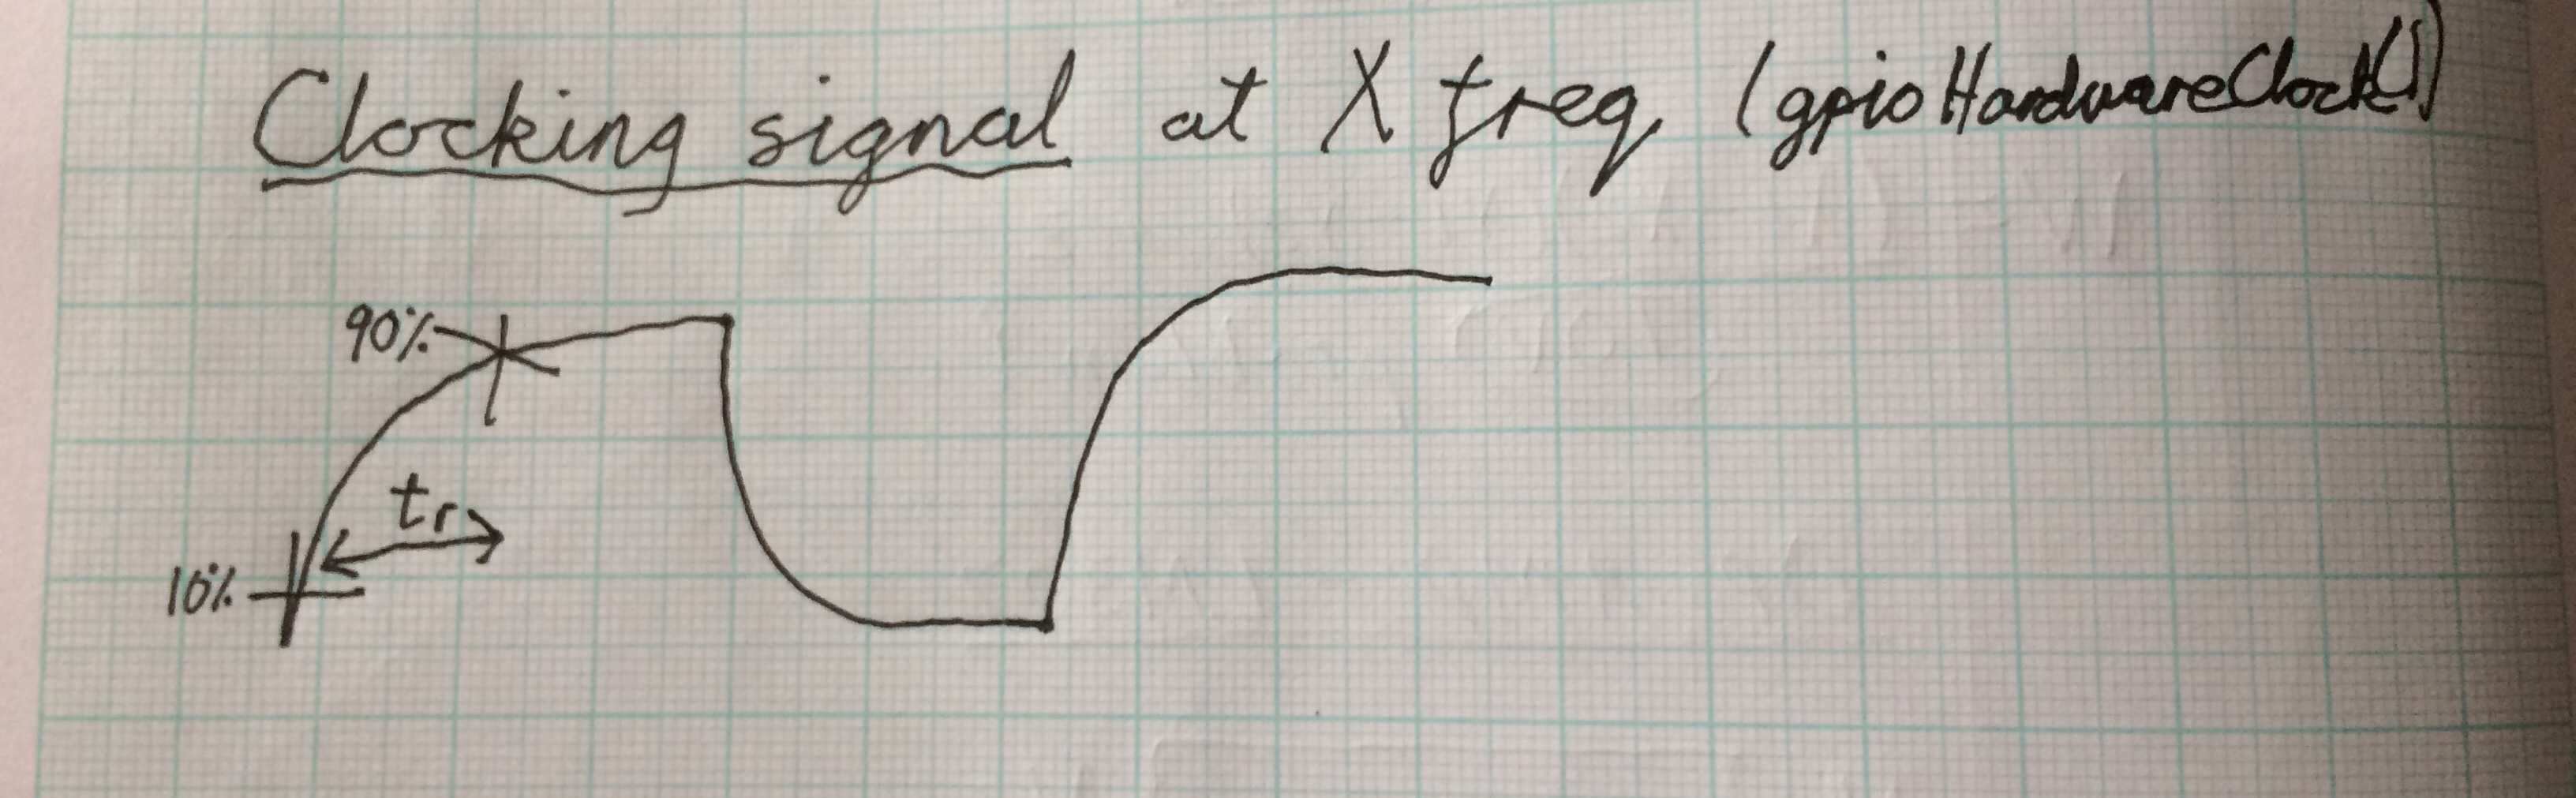
\includegraphics[width=0.6\textwidth]{Clock_Analyse.jpg}
	\caption{This is a high frequency view of the hardware clock for interest and rise-time (max frequency achievable actually)}
	%\label{fig_}
\end{figure}

\subsection{Comparing Python and C} \label{sec_Comparing Python and C}

%%%%%%%%%%%%%%%%%%%%%%%%%%%%%%%%%%%%%%%%%%%%%%%%%%%%%%%%%%%%%%%%%%%%%%%%%%%%%%%%%%%%%%%%%%%%%%%%%%%%%%%%%%%%%%%%%%%%%%%%%%%%%%%%%%

\section{Characterising Components of the Test Bed} \label{sec_Components}

\begin{figure}[ht]
	\centering
	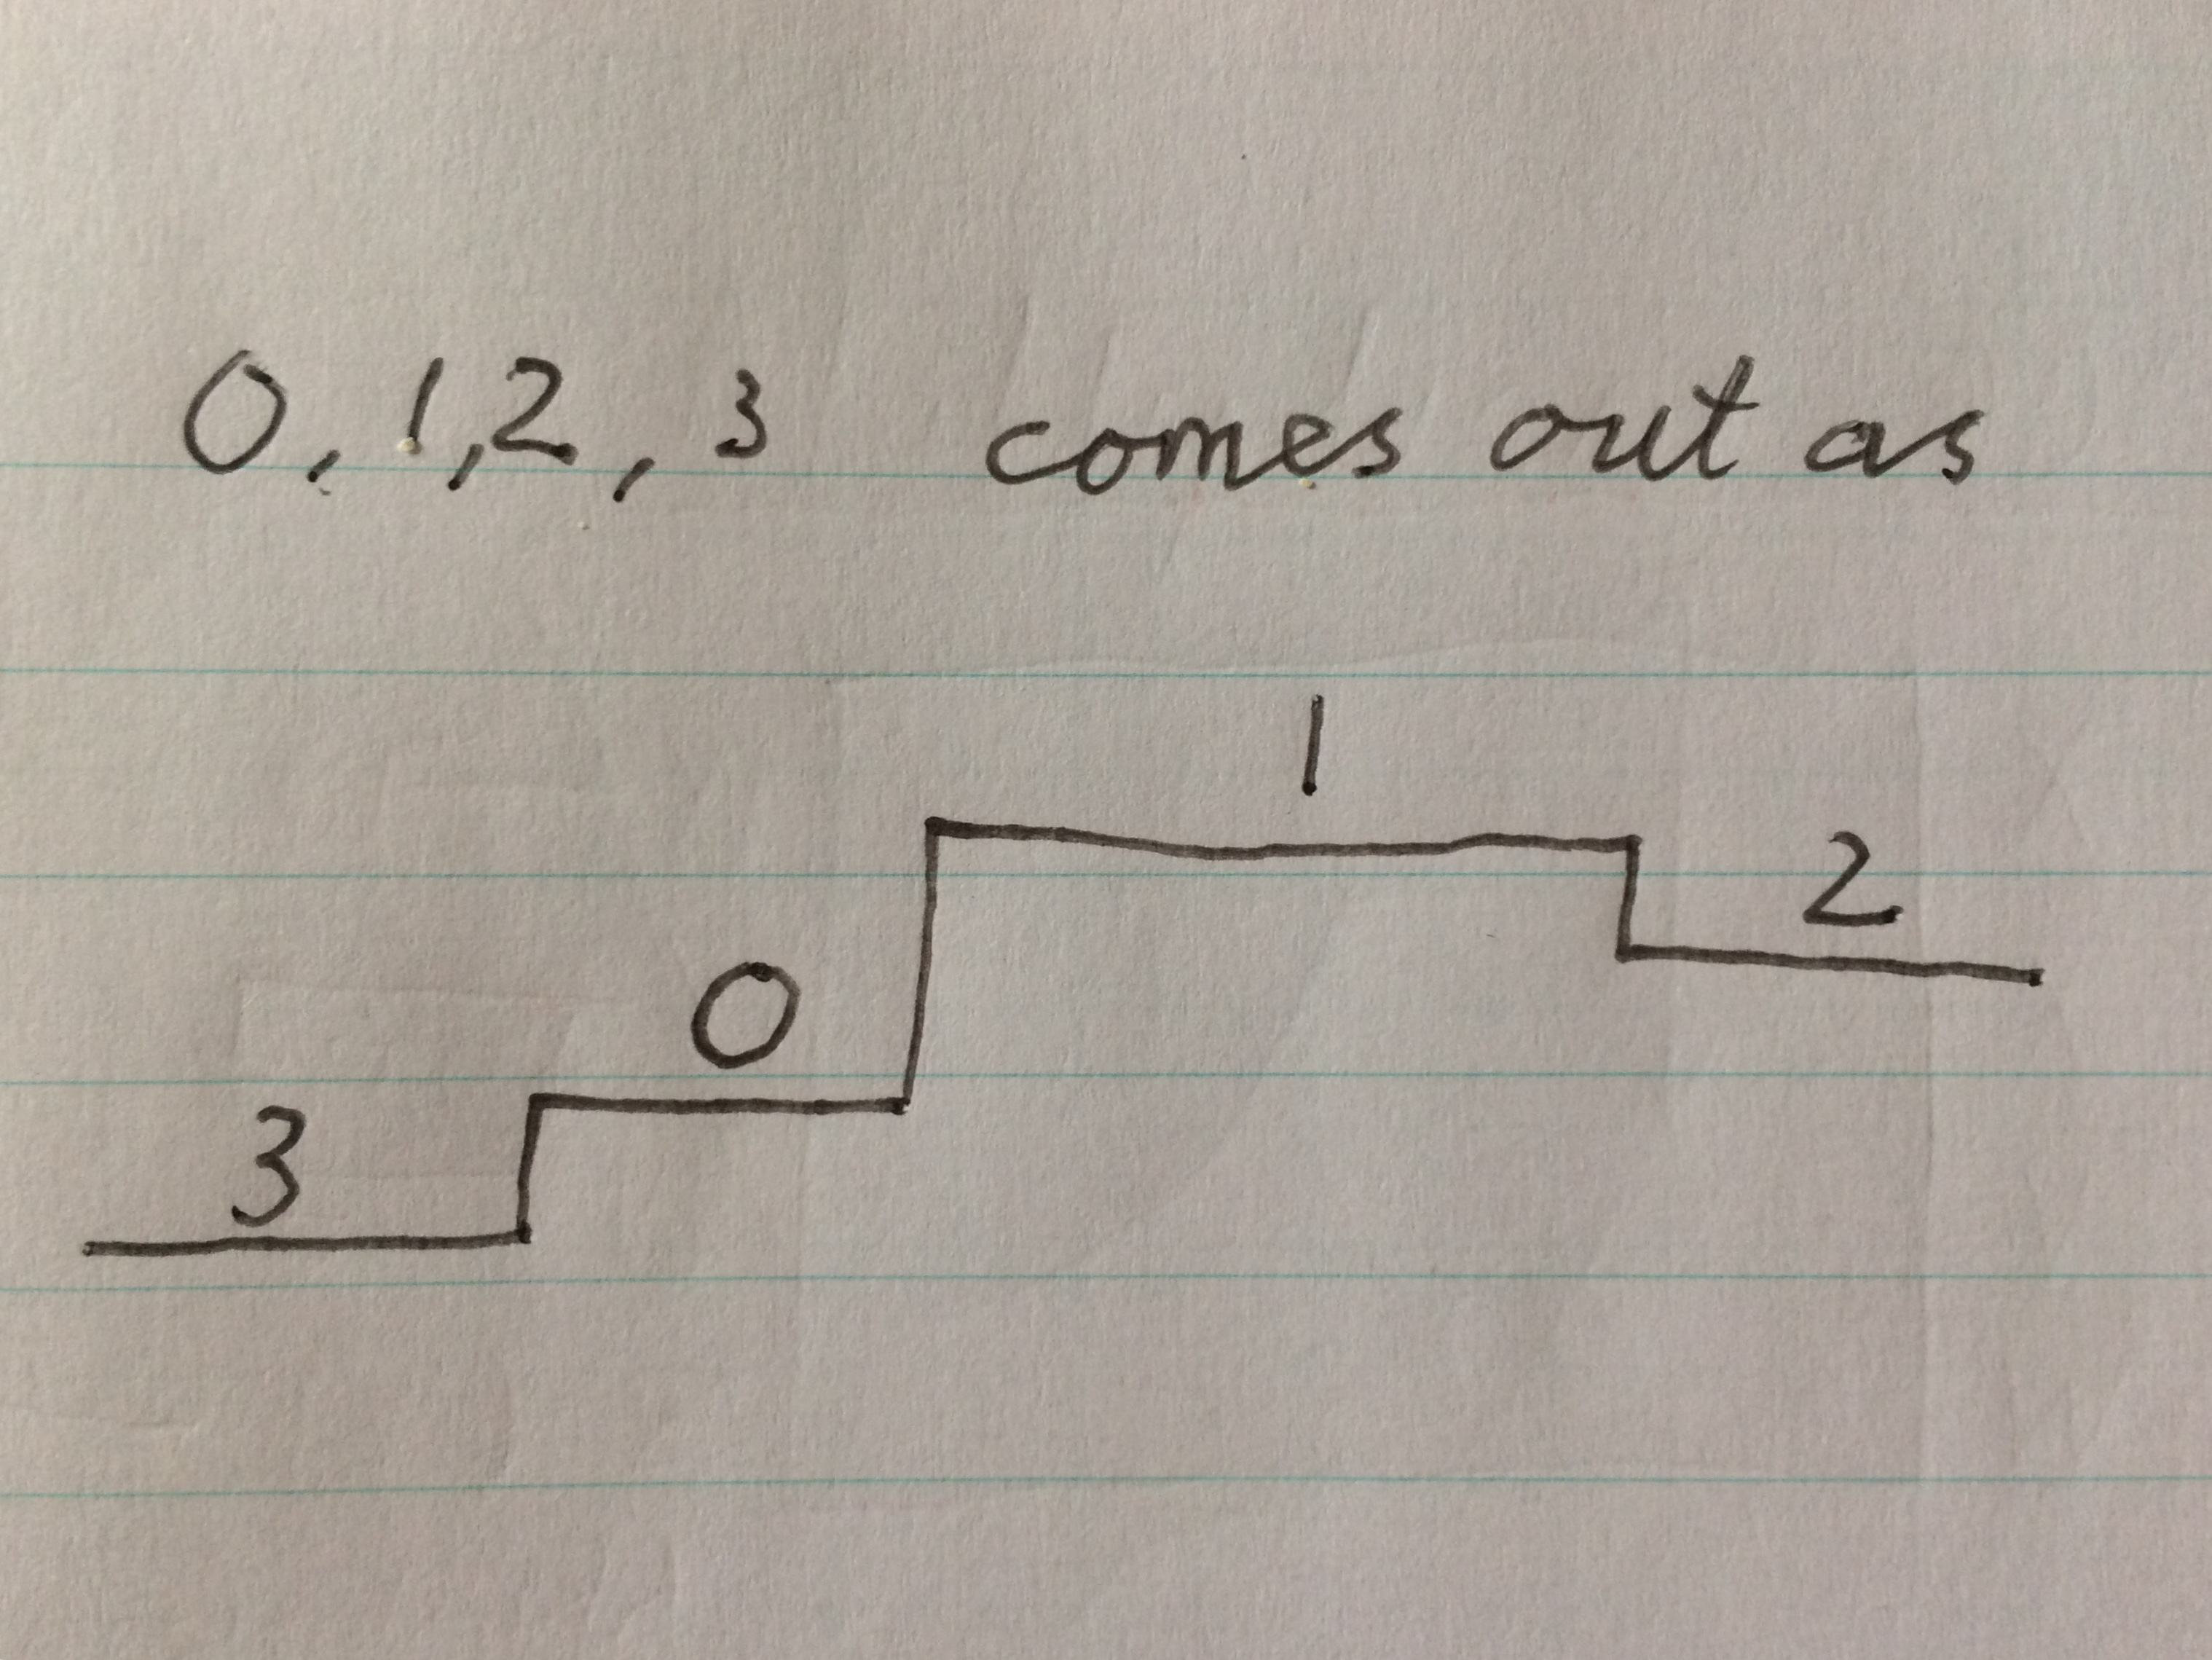
\includegraphics[width=0.6\textwidth]{DAC_Output.jpg}
	\caption{Non-continuous Output for Continuous Input Values of the DAC}
	%\label{fig_}
\end{figure}

\begin{figure}[ht]
	\centering
	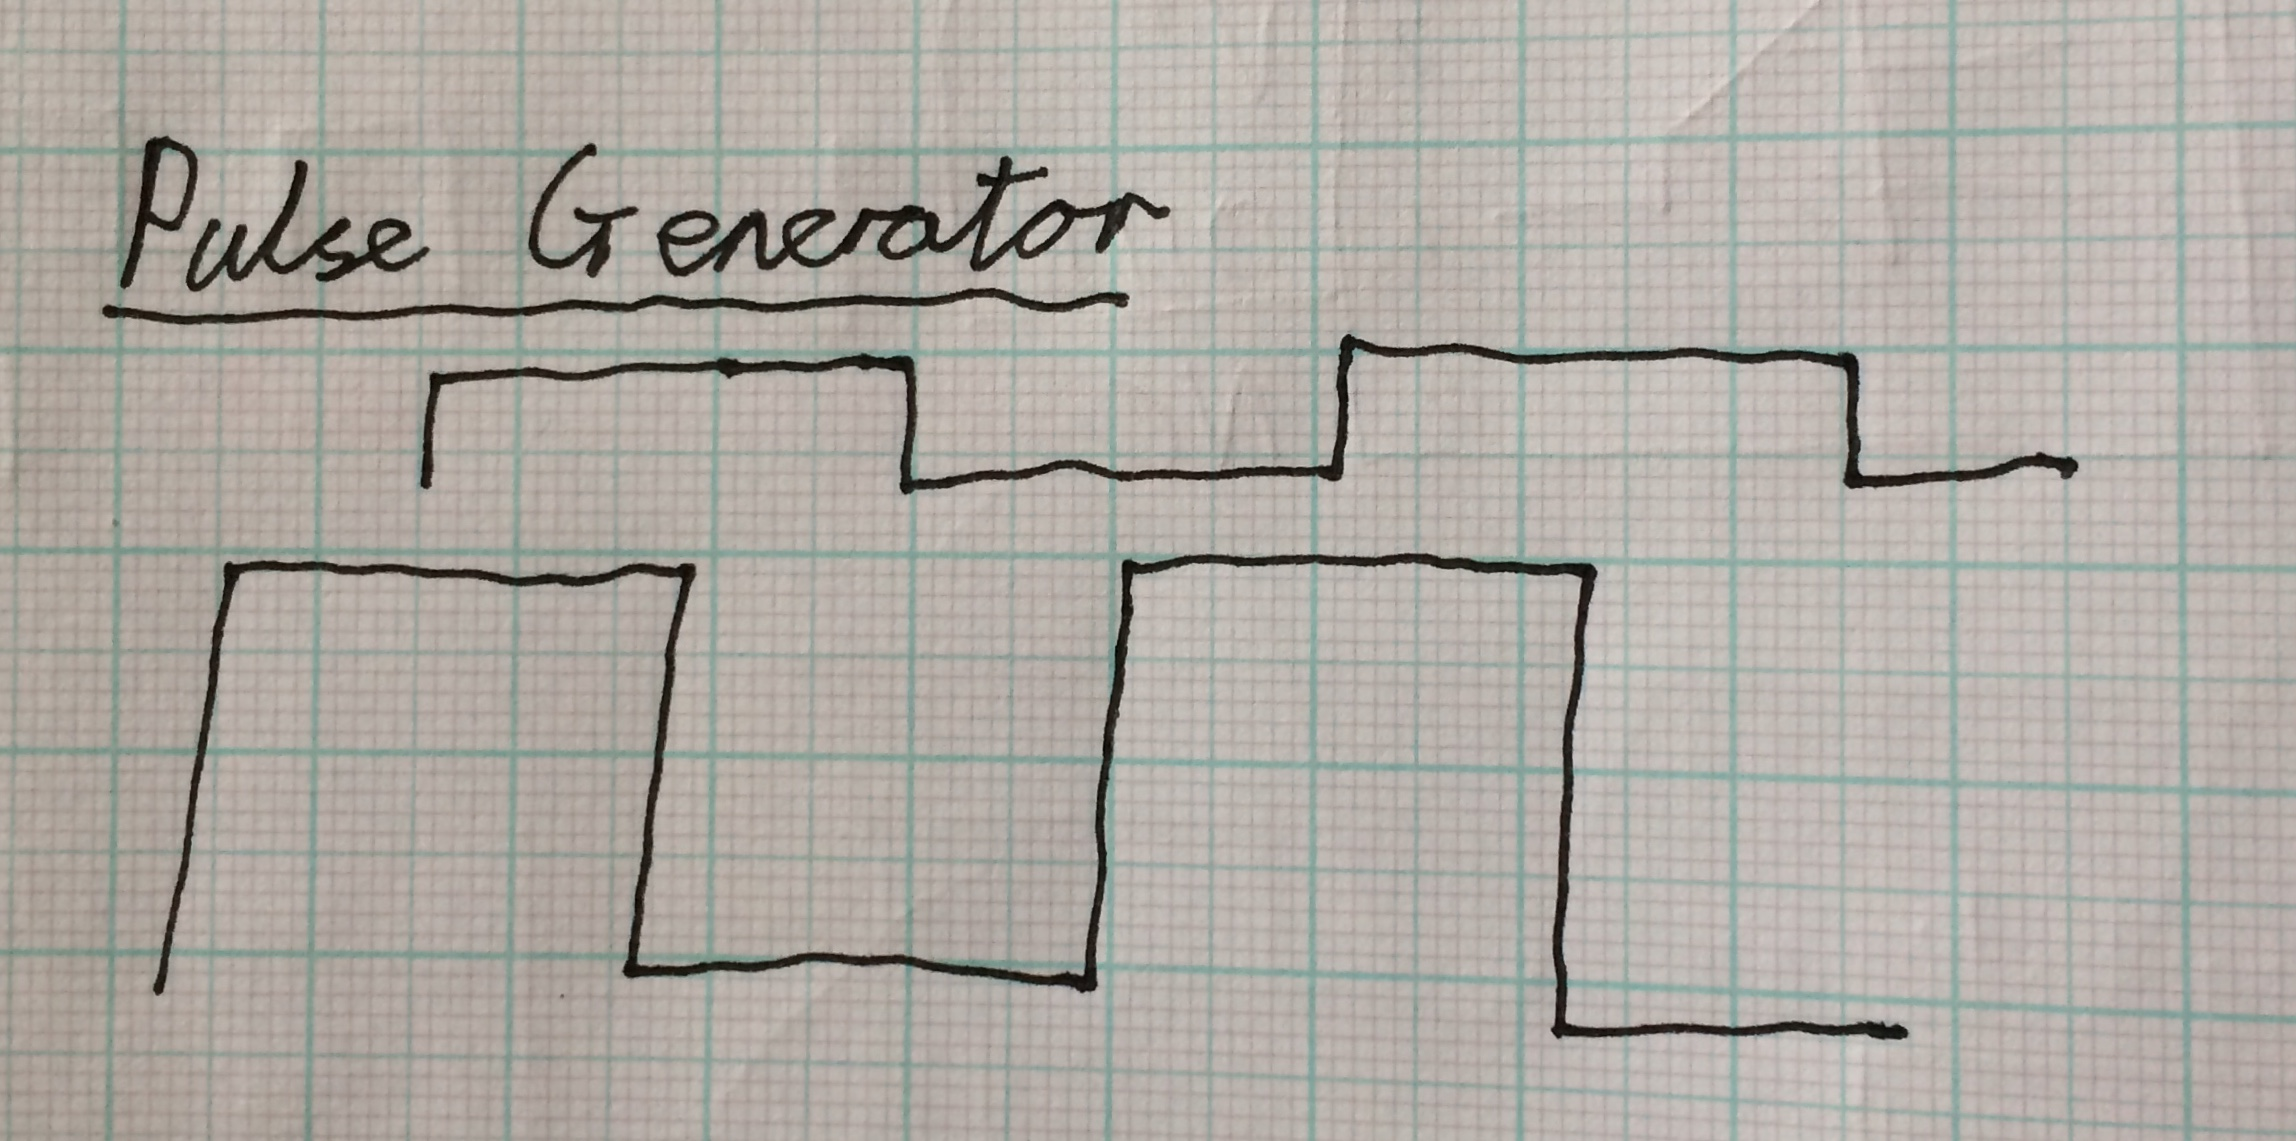
\includegraphics[width=0.6\textwidth]{Pulse_Output.jpg}
	\caption{Output of pulse generator}
	%\label{fig_}
\end{figure}

\begin{figure}[ht]
	\centering
	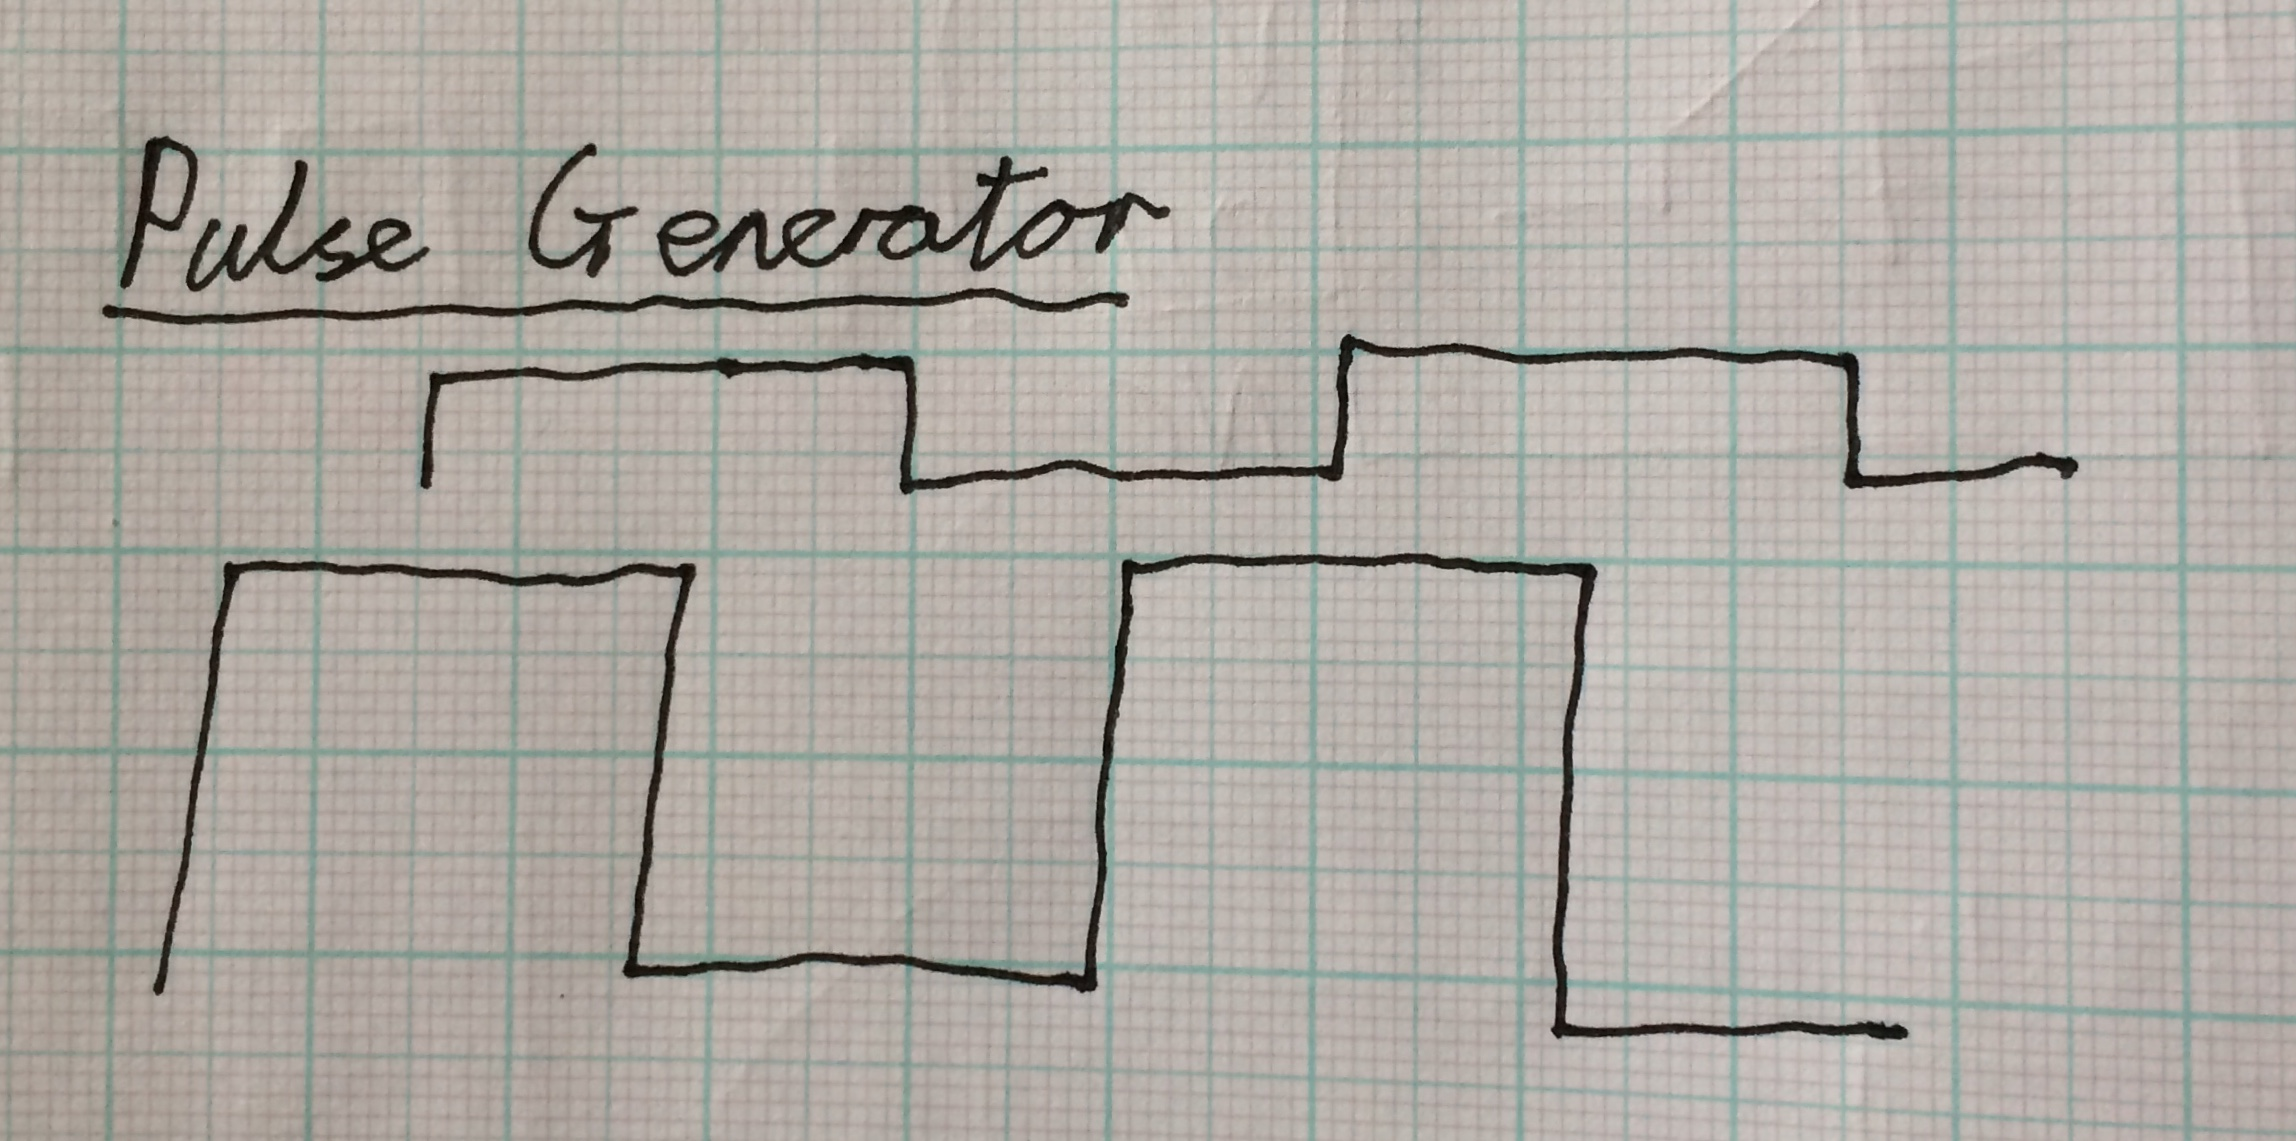
\includegraphics[width=0.6\textwidth]{Pulse_Output.jpg}
	\caption{Output of pulse generator once filtered to be sine waves}
	%\label{fig_}
\end{figure}



Electrical Components:
\begin{itemize}
	\item Analogue Digital Converter
	\item Digital Analogue Converter
	\item Quadrature Sinusoid Generator
	\item Multiplier/Mixer
	\item Low Pass Filters
\end{itemize}

\subsection{Overclocking Components}

\end{document}